% !TEX program = lualatex
\documentclass[../../main.tex]{subfiles}
\begin{document}


\begin{figure}[h]
	\centering

	\subfloat[][Bottom]{
		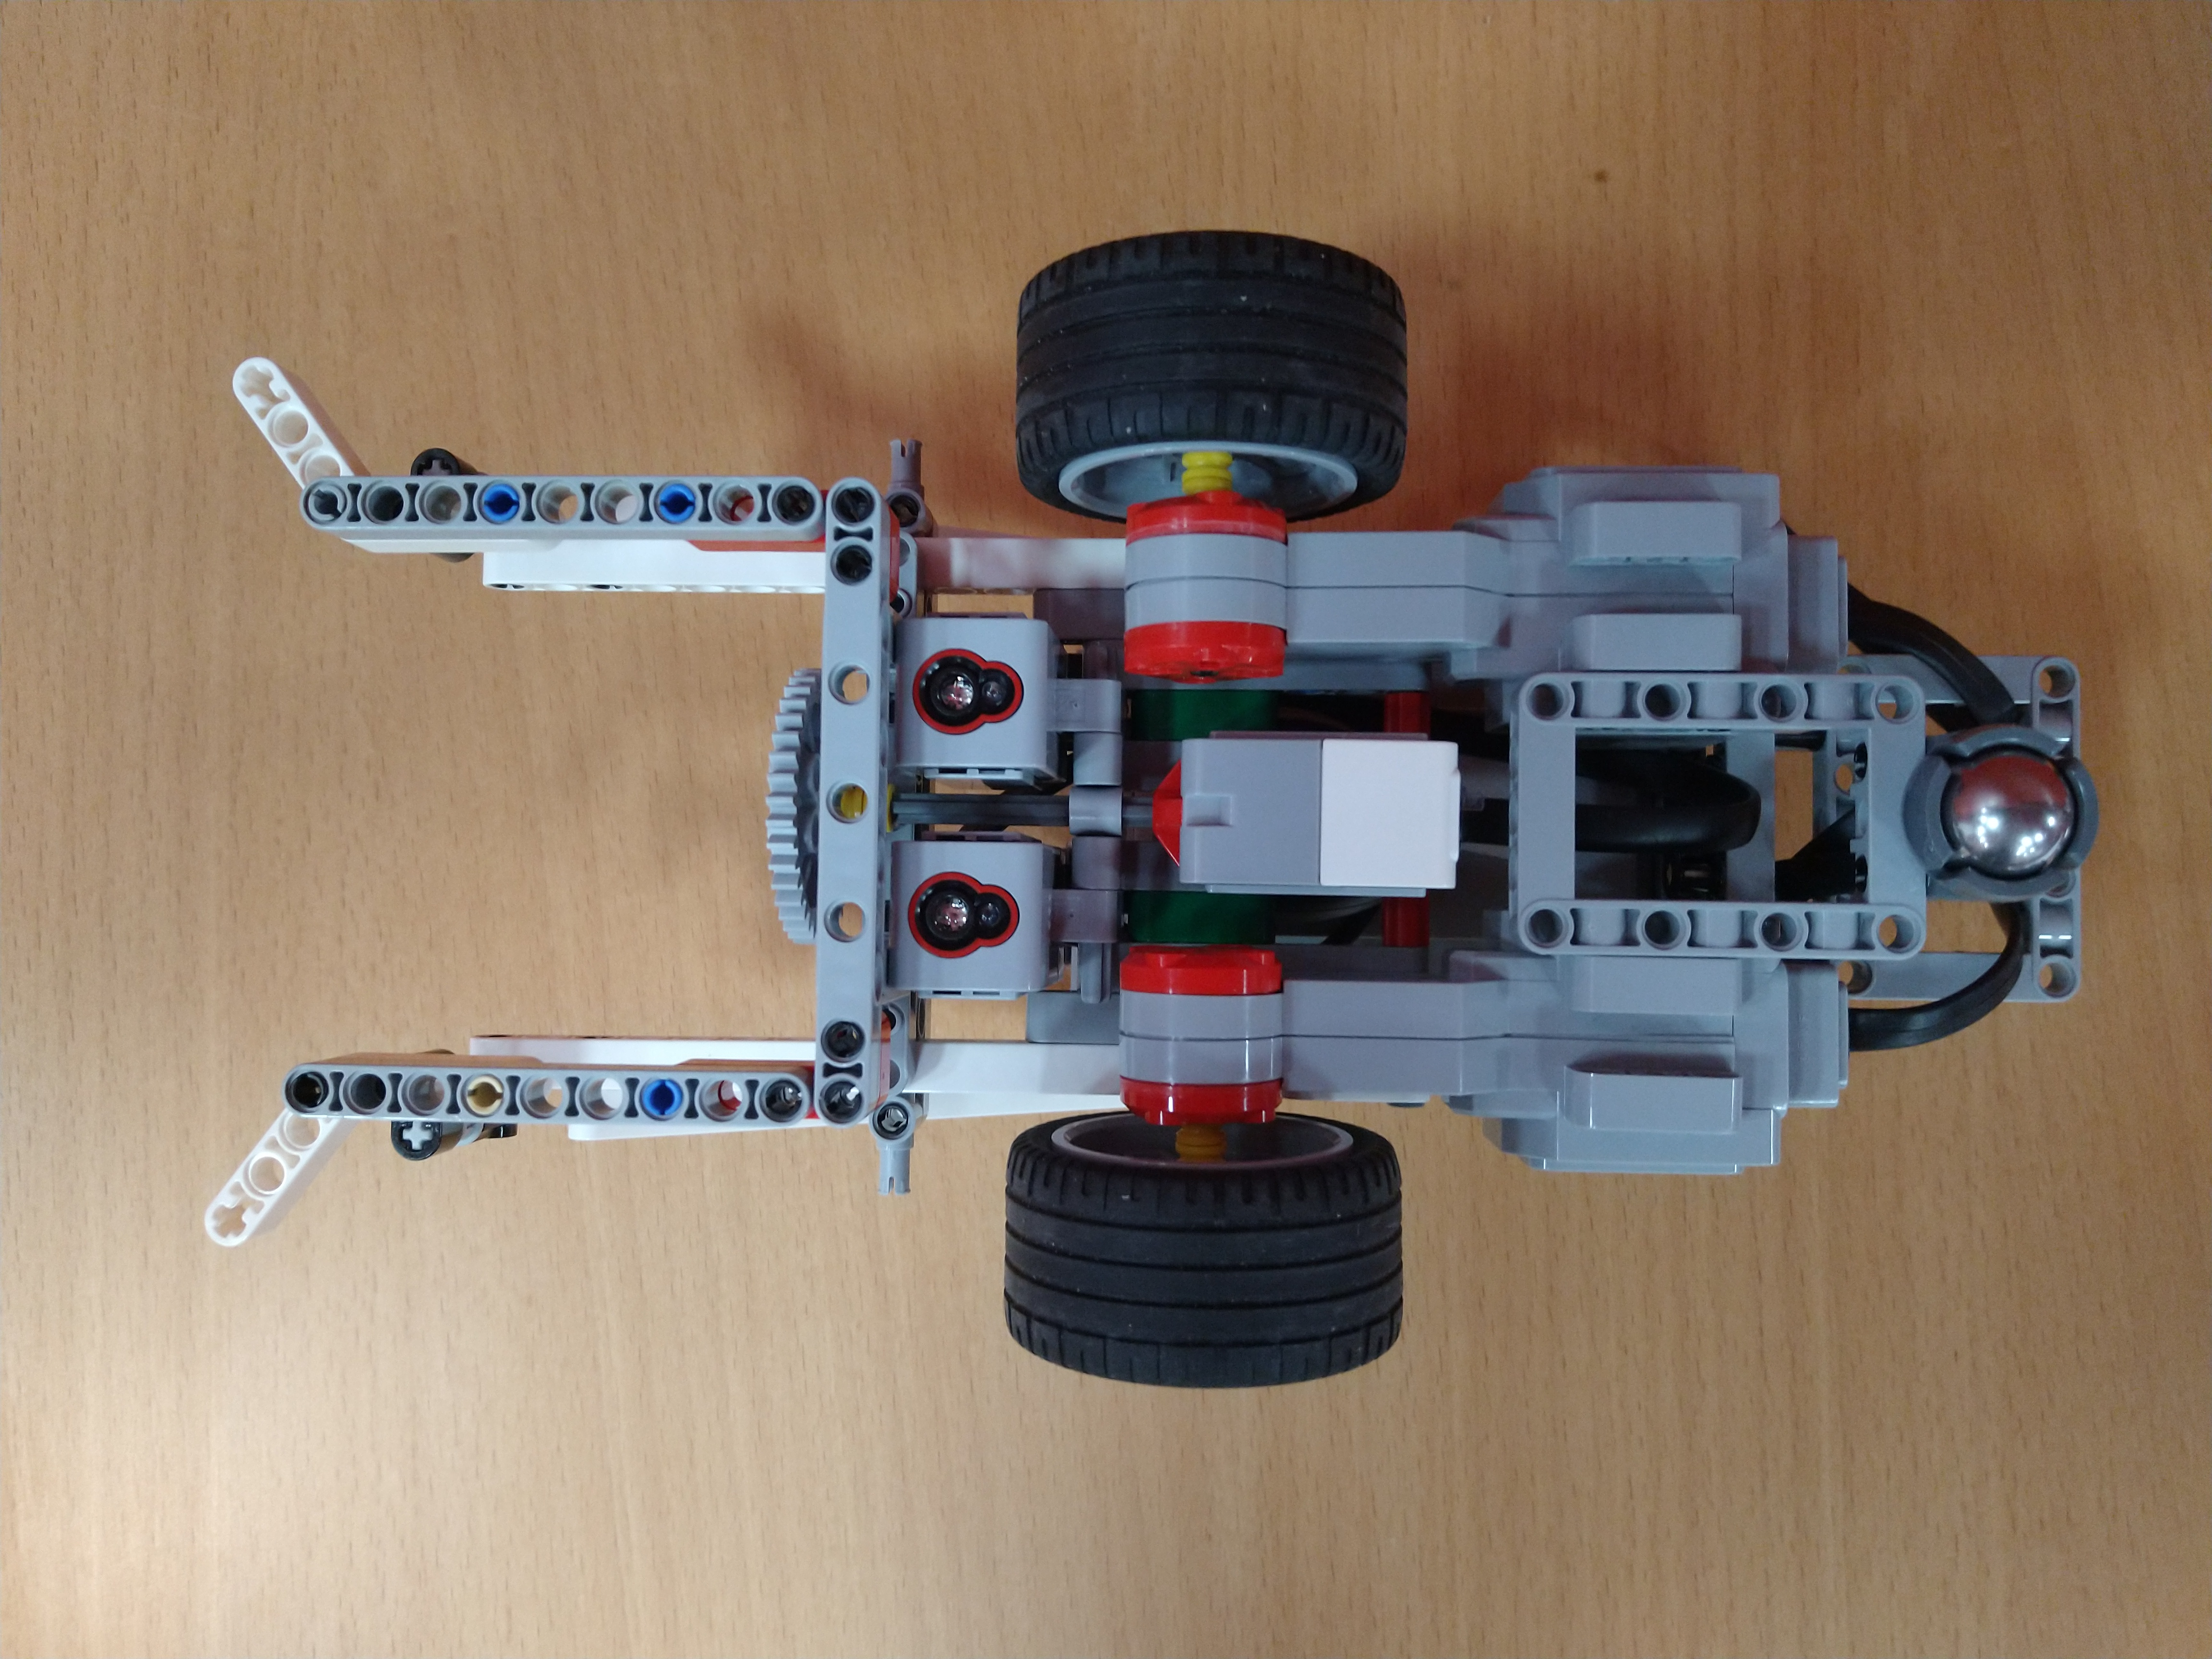
\includegraphics[width=0.4\linewidth]{images/bottom.jpg}
	\label{fig:images/bottom}
	}
	\subfloat[][Front]{
		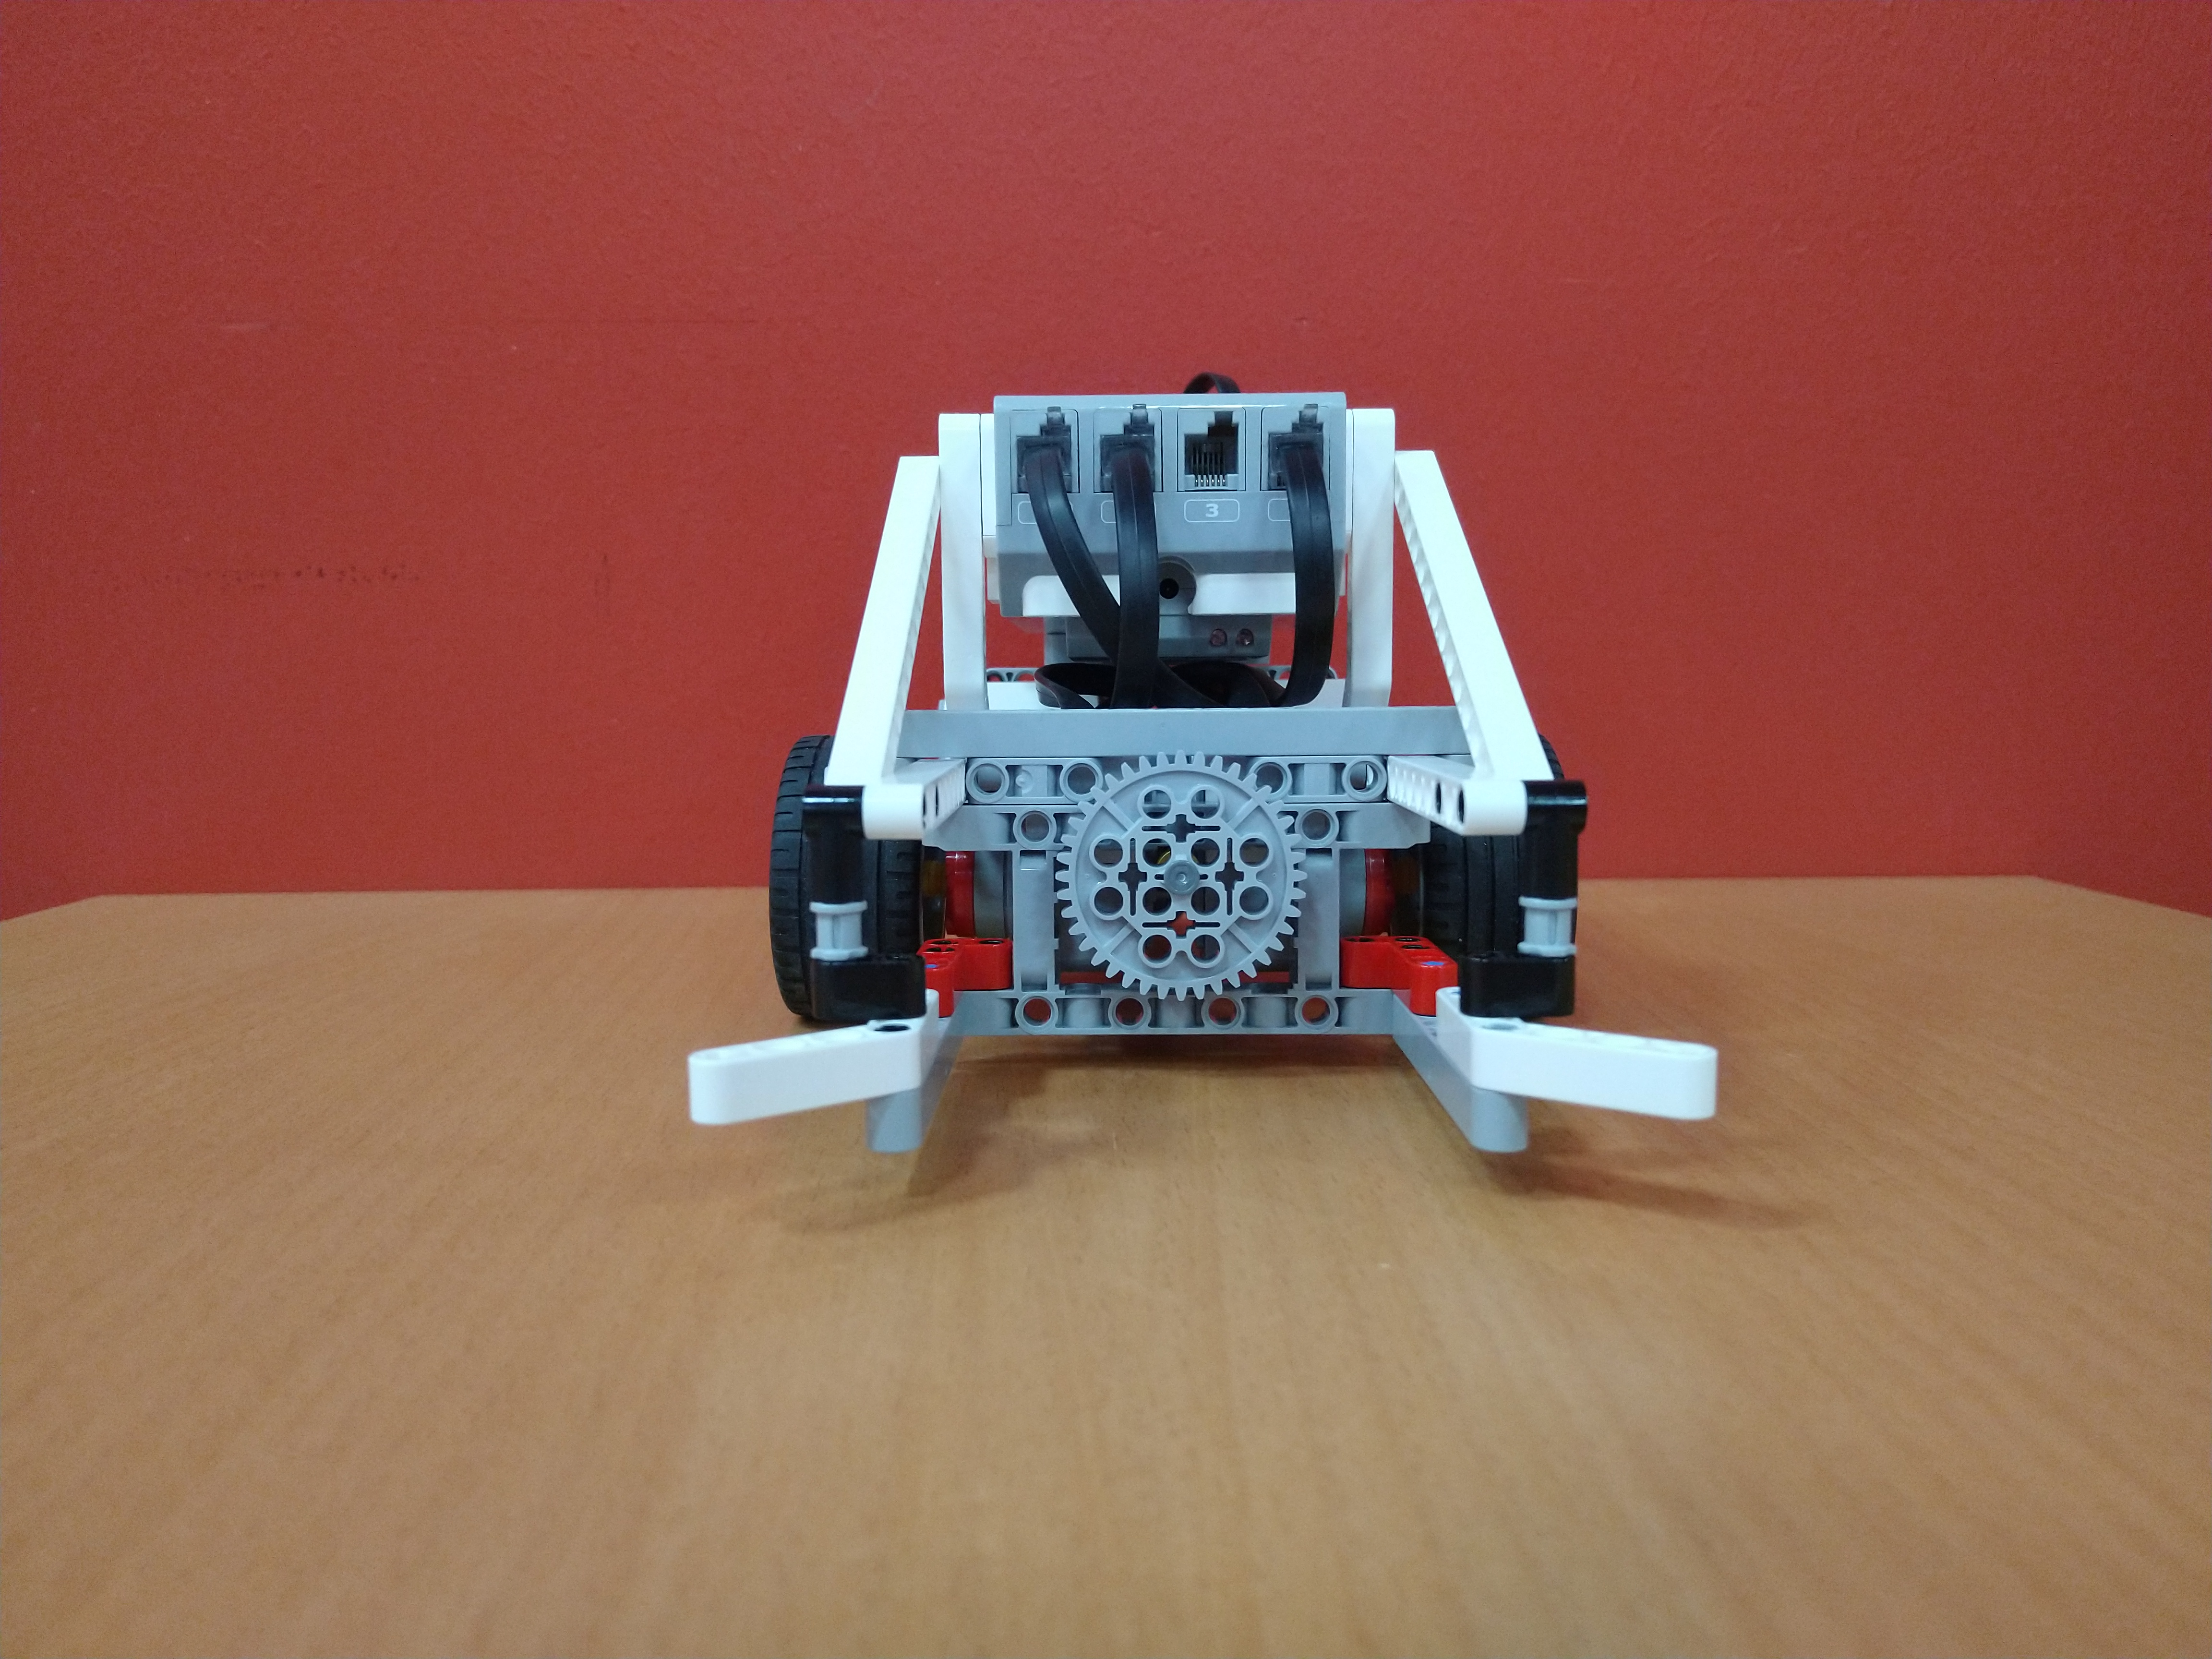
\includegraphics[width=0.4\linewidth]{images/front.jpg}
	\label{fig:images/front}
	}
	\caption{Bottom and Front of ev3 robot}
	\label{fig:front_and_bottom}
\end{figure}


In general the robot is made as compact as possible.\\


To sense the map the color sensors are placed far enough apart to allow a line between them.
This is to ensure that the root will not jitter and constantly correct its course while
following the map.

The sensors can be seen on figure \subref{fig:images/bottom}.

To sense the can, a pressure sensor is mounted in the cage of the robot, as can be seen in figure
\subref{fig:images/bottom}. To best detect the can the pressure sensors surface is increased by using
a cog, as can be seen on figure \subref{fig:images/front}.\\

The robot also able "sense" how far it has moving via the encoders int the motors.\\

To navigate the map the robot relies on odometry and the color sensors to correct drift.
This limited sensing requires the robot to know its starting position. It also makes difficult
to recover if lost.\\

To account for the cans or the robot  not being in the exactly the right place, the inlet on the cage
is wider than the cage itself. And also the pressure sensors will detect when the robot makes 
contact with the can.
	
\end{document}
